%% Run LaTeX on this file several times to get Table of Contents,
%% cross-references, and citations.

\documentclass[11pt]{book}
\usepackage{gvv}
\usepackage{gvv-book-bkup}
%\usepackage{Wiley-AuthoringTemplate}
\usepackage[sectionbib,authoryear]{natbib}% for name-date citation comment the below line
%\usepackage[sectionbib,numbers]{natbib}% for numbered citation comment the above line

%%********************************************************************%%
%%       How many levels of section head would you like numbered?     %%
%% 0= no section numbers, 1= section, 2= subsection, 3= subsubsection %%
\setcounter{secnumdepth}{3}
%%********************************************************************%%
%%**********************************************************************%%
%%     How many levels of section head would you like to appear in the  %%
%%				Table of Contents?			%%
%% 0= chapter, 1= section, 2= subsection, 3= subsubsection titles.	%%
\setcounter{tocdepth}{2}
%%**********************************************************************%%

%\includeonly{ch01}
\makeindex

\begin{document}

\frontmatter
%%%%%%%%%%%%%%%%%%%%%%%%%%%%%%%%%%%%%%%%%%%%%%%%%%%%%%%%%%%%%%%%
%% Title Pages
%% Wiley will provide title and copyright page, but you can make
%% your own titlepages if you'd like anyway
%% Setting up title pages, type in the appropriate names here:

\booktitle{CBSE Math}

\subtitle{Made Simple}

\AuAff{G. V. V. Sharma}


%% \\ will start a new line.
%% You may add \affil{} for affiliation, ie,
%\authors{Robert M. Groves\\
%\affil{Universitat de les Illes Balears}
%Floyd J. Fowler, Jr.\\
%\affil{University of New Mexico}
%}

%% Print Half Title and Title Page:
%\halftitlepage
\titlepage

%%%%%%%%%%%%%%%%%%%%%%%%%%%%%%%%%%%%%%%%%%%%%%%%%%%%%%%%%%%%%%%%
%% Copyright Page

\begin{copyrightpage}{2023}
%Title, etc
\end{copyrightpage}

% Note, you must use \ to start indented lines, ie,
% 
% \begin{copyrightpage}{2004}
% Survey Methodology / Robert M. Groves . . . [et al.].
% \       p. cm.---(Wiley series in survey methodology)
% \    ``Wiley-Interscience."
% \    Includes bibliographical references and index.
% \    ISBN 0-471-48348-6 (pbk.)
% \    1. Surveys---Methodology.  2. Social 
% \  sciences---Research---Statistical methods.  I. Groves, Robert M.  II. %
% Series.\\

% HA31.2.S873 2004
% 001.4'33---dc22                                             2004044064
% \end{copyrightpage}

%%%%%%%%%%%%%%%%%%%%%%%%%%%%%%%%%%%%%%%%%%%%%%%%%%%%%%%%%%%%%%%%
%% Only Dedication (optional) 

%\dedication{To my parents}

\tableofcontents

%\listoffigures %optional
%\listoftables  %optional

%% or Contributor Page for edited books
%% before \tableofcontents

%%%%%%%%%%%%%%%%%%%%%%%%%%%%%%%%%%%%%%%%%%%%%%%%%%%%%%%%%%%%%%%%
%  Contributors Page for Edited Book
%%%%%%%%%%%%%%%%%%%%%%%%%%%%%%%%%%%%%%%%%%%%%%%%%%%%%%%%%%%%%%%%

% If your book has chapters written by different authors,
% you'll need a Contributors page.

% Use \begin{contributors}...\end{contributors} and
% then enter each author with the \name{} command, followed
% by the affiliation information.

% \begin{contributors}
% \name{Masayki Abe,} Fujitsu Laboratories Ltd., Fujitsu Limited, Atsugi, Japan
%
% \name{L. A. Akers,} Center for Solid State Electronics Research, Arizona State University, Tempe, Arizona
%
% \name{G. H. Bernstein,} Department of Electrical and Computer Engineering, University of Notre Dame, Notre Dame, South Bend, Indiana; formerly of
% Center for Solid State Electronics Research, Arizona
% State University, Tempe, Arizona 
% \end{contributors}

%%%%%%%%%%%%%%%%%%%%%%%%%%%%%%%%%%%%%%%%%%%%%%%%%%%%%%%%%%%%%%%%
% Optional Foreword:

%\begin{foreword}
%\lipsum[1-2]
%\end{foreword}

%%%%%%%%%%%%%%%%%%%%%%%%%%%%%%%%%%%%%%%%%%%%%%%%%%%%%%%%%%%%%%%%
% Optional Preface:

%\begin{preface}
%\lipsum[1-1]
%\prefaceauthor{}
%\where{place\\
% date}
%\end{preface}

% ie,
% \begin{preface}
% This is an example preface.
% \prefaceauthor{R. K. Watts}
% \where{Durham, North Carolina\\
% September, 2004}

%%%%%%%%%%%%%%%%%%%%%%%%%%%%%%%%%%%%%%%%%%%%%%%%%%%%%%%%%%%%%%%%
% Optional Acknowledgments:

%\acknowledgments
%\lipsum[1-2]
%\authorinitials{I. R. S.}  

%%%%%%%%%%%%%%%%%%%%%%%%%%%%%%%%
%% Glossary Type of Environment:

% \begin{glossary}
% \term{<term>}{<description>}
% \end{glossary}

%%%%%%%%%%%%%%%%%%%%%%%%%%%%%%%%
%\begin{acronyms}
%\acro{ASTA}{Arrivals See Time Averages}
%\acro{BHCA}{Busy Hour Call Attempts}
%\acro{BR}{Bandwidth Reservation}
%\acro{b.u.}{bandwidth unit(s)}
%\acro{CAC}{Call / Connection Admission Control}
%\acro{CBP}{Call Blocking Probability(-ies)}
%\acro{CCS}{Centum Call Seconds}
%\acro{CDTM}{Connection Dependent Threshold Model}
%\acro{CS}{Complete Sharing}
%\acro{DiffServ}{Differentiated Services}
%\acro{EMLM}{Erlang Multirate Loss Model}
%\acro{erl}{The Erlang unit of traffic-load}
%\acro{FIFO}{First in - First out}
%\acro{GB}{Global balance}
%\acro{GoS}{Grade of Service}
%\acro{ICT}{Information and Communication Technology}
%\acro{IntServ}{Integrated Services}
%\acro{IP}{Internet Protocol}
%\acro{ITU-T}{International Telecommunication Unit -- Standardization sector}
%\acro{LB}{Local balance}
%\acro{LHS}{Left hand side}
%\acro{LIFO}{Last in - First out}
%\acro{MMPP}{Markov Modulated Poisson Process}
%\acro{MPLS}{Multiple Protocol Labeling Switching}
%\acro{MRM}{Multi-Retry Model}
%\acro{MTM}{Multi-Threshold Model}
%\acro{PASTA}{Poisson Arrivals See Time Averages}
%\acro{PDF}{Probability Distribution Function}
%\acro{pdf}{probability density function}
%\acro{PFS}{Product Form Solution}
%\acro{QoS}{Quality of Service}
%\acro{r.v.}{random variable(s)}
%\acro{RED}{random early detection}
%\acro{RHS}{Right hand side}
%\acro{RLA}{Reduced Load Approximation}
%\acro{SIRO}{service in random order}
%\acro{SRM}{Single-Retry Model}
%\acro{STM}{Single-Threshold Model}
%\acro{TCP}{Transport Control Protocol}
%\acro{TH}{Threshold(s)}
%\acro{UDP}{User Datagram Protocol}
%\end{acronyms}

\setcounter{page}{1}

\begin{introduction}
This book links high school coordinate geometry to linear algebra and matrix analysis through solved problems.

\end{introduction}

\mainmatter
\chapter{Vectors}
\section{2023}
\subsection{10}
\input{2023/vectors10-1.tex}
\subsection{12}
\input{2023/vector12-1.tex}
\section{2022}
\subsection{10}
\begin{enumerate}[label=\thesection.\arabic*.,ref=\thesection.\theenumi]
\numberwithin{equation}{enumi}
\numberwithin{figure}{enumi}
\numberwithin{table}{enumi} 
\item The distance between the points $(0,0)$ and $(a-b, a+b)$ is 
\begin{enumerate}
\item $2{\sqrt{ab}}$
\item $\sqrt{2a^2 + ab}$
\item $ 2\sqrt{a^2 + b^2}$
\item $ \sqrt{2a^2 + 2b^2}$
\end{enumerate}
\item The value of m which makes the point $(0,0)$ , $(2m, -4)$ and $(3,6)$ collinear, is $\underline{\hspace{1cm}}$
\item A circle has its center at $(4,4)$. If one end of a diameter is $(4,0)$, then find the coordinates of other end.
\item  Find the area of the quadrilateral ABCD whose vertices are $\vec A(-4, -3)$ , $\vec B(3, -1)$, $\vec C(0, 5)$ and $\vec D(-4, 2)$
\item If the points $\vec{A}(2,0)$, $\vec{B}(6,1)$, and $\vec{C}(p ,q)$ form a triangle of area 12sq. units (positive only) and \begin{align}2p + q = 10\end{align}, then find the values of p and q.
\end{enumerate}


\subsection{12}
\begin{enumerate}
\item $\overrightarrow{a}$   and  $\overrightarrow{ b}$ are two unit vectors such that \begin{align} \abs { 2\overrightarrow{ a}+3\overrightarrow{ b}} = \abs{3\overrightarrow{ a} - 2\overrightarrow{ b}}. \end{align} Find the angle between $\overrightarrow{ a }$ and $\overrightarrow{ b }$.
\item If $\overrightarrow{ a}$  and $\overrightarrow{b}$ are two vectors such that  \begin{align}\overrightarrow{a} = \hat{i} - \hat{j} + \hat{k} \end{align}and  \begin{align}\overrightarrow{b} = 2\hat{i} - \hat{j} - 3\hat{k}\end{align} then find the vector $\overrightarrow{c}$, given that \begin{align}\overrightarrow{a} \times \overrightarrow{c} = \overrightarrow{b}\end{align}  and \begin{align}\overrightarrow{a}.\overrightarrow{c}= 4.\end{align}
\item \begin{align} If \abs{\overrightarrow{ a } \times \overrightarrow { b }}^2 + \abs { \overrightarrow{ a } . \overrightarrow{ b }}^2= 400 \end{align} and  \begin{align}\abs { \overrightarrow{ b}} = 5 \end{align} find the value of  $\abs{\overrightarrow{ a }}$. 
\item If \begin{align}\overrightarrow{a} = \hat{i} + \hat{ j} + \hat{ k} , \overrightarrow{a} . \overrightarrow{b} = 1\end{align}  and \begin{align}\overrightarrow{a} \times \overrightarrow{b} = \hat{j} - \hat{k}\end{align},  then find  $\abs{\overrightarrow{b}}$ 
\item If \begin{align}\abs{\overrightarrow{ a}}= 3, \abs{\overrightarrow{ b}} = 2\sqrt{ 3}\end{align}  and \begin{align}\overrightarrow{ a} . \overrightarrow{ b} = 6,\end{align}then find the value of $\abs{\overrightarrow{ a} \times \overrightarrow{ b}}$.
\item $\abs{\overrightarrow{a}} = 8, \abs{\overrightarrow{ b}} = 3$ and $\overrightarrow{a} . \overrightarrow{b} = 12\sqrt{3}$, then the value of  $\abs{\overrightarrow{a} \times \overrightarrow{b}}$ is
\begin{enumerate}                                      
\item  24                                              
\item  144                                             
\item  2                                              
\item  12                                             
\end{enumerate}
\item If$\space$ \begin{align}\overrightarrow{ a} = 2\hat{i} + \hat{j} + 3\hat{k}, \hat{b} = -\hat{i} + 2\hat{j} + \hat{k}\end{align} and \begin{align}\overrightarrow{c} = 3\hat{i} + \hat{j} + 2\hat{k}\end{align}, then find $\overrightarrow{a} . (\overrightarrow{ b} \times \overrightarrow{c})$. 
	\item $\overrightarrow{a}, \overrightarrow{ b },\overrightarrow{ c }$  and  $\overrightarrow{ d }$ are four non-zeros vectors such that  \begin{align}\overrightarrow{a}\times \overrightarrow{b}= \overrightarrow{c} \times \overrightarrow{d}\end{align}  and  \begin{align}\overrightarrow{a} \times \overrightarrow{c} = 4\overrightarrow{b} \times \overrightarrow{d}\end{align}, then show that  $(\overrightarrow{ a}-2\overrightarrow{d})$ \text{ is parallel to} $(2\overrightarrow{b}-\overrightarrow{c})$ where \begin{align}\overrightarrow{a} \neq 2\overrightarrow{d}, \overrightarrow{c} \neq 2\overrightarrow{b}\end{align}
\item If \begin{align}\overrightarrow{a} = \hat{i} + \hat{ j} + \hat{ k} , \overrightarrow{a} . \overrightarrow{b} = 1\end{align}  and \begin{align}\overrightarrow{a} \times \overrightarrow{b} = \hat{j} - \hat{k},\end{align}  then find  $\abs{\overrightarrow{b}}$
\item  If $\overrightarrow{ a}$  and  $\overrightarrow{b}$  are two vectors such that \begin{align}\abs{\overrightarrow{a} + \overrightarrow{b}} = \abs{ \overrightarrow{b}},\end{align}then prove that $(\overrightarrow{a} + 2\overrightarrow{b})$  is perpendicular to $\overrightarrow{ a}$.
\item If $\overrightarrow{ a}$ and $\overrightarrow{ b}$ are unit vectors and $\theta$ is the angle between them , then prove that sin \begin{align}\frac{\theta}{ 2} = \frac{1}{2}\abs{\overrightarrow{ a} - \overrightarrow{ b}}\end{align}
\item If $\overrightarrow{a}$ and $\overrightarrow{b}$  are two unit vectors such that and $\theta$ is the angle between them, then prove that                       \begin{align}sin \dfrac{ \theta}{2} = \frac{1}{2} \abs{\overrightarrow{a} - \overrightarrow{b}} \end{align} 
\item If \begin{align}\overrightarrow{a} = 2\hat{i} + y\hat{j} + \hat{ k}\end{align} and \begin{align}\overrightarrow{ b} = \hat{i} + 2\hat{j}+ 3\hat{k}\end{align} are two vectors for which the vector $(\overrightarrow{a}+\overrightarrow{b})$ is perpendicular to the vector  $(\overrightarrow{a}-\overrightarrow{b})$ then find all the possible values of y.
\item Write the projection of the vector $(\overrightarrow{b}+\overrightarrow{c})$  on the vector  $\overrightarrow{a}$ ,  where \begin{align}\overrightarrow{ a} = 2\hat{i}-2\hat{j}+\hat{k}, \overrightarrow{b} = \hat{i}+2\hat{j}-2\hat{k}\end{align} and \begin{align}\overrightarrow{c} = 2\hat{i}-\hat{j}+4\hat{k}.\end{align}
\item If \begin{align}\overrightarrow{ a } = 2\hat{i} - \hat{ j } +\hat{ k }, \overrightarrow{ b } = \hat{ i } + \hat{ j} - 2\hat{ k }\end{align} and  \begin{align}\overrightarrow{ c } = \hat{ i } +3\hat{j} - \hat{k}\end{align} and the projection of vector   $\overrightarrow{c} + \lambda \overrightarrow{b}$  on  vector  $\overrightarrow{a}$  is $2\sqrt{6}$, find the value of $\lambda$.
	\item If \begin{align}\overrightarrow{ a} = 2\hat{i} + \hat {j} +3\hat{k}, \hat{b} = -\hat{i} + 2\hat{j} + \hat{k }\end{align} and  \begin{align}\overrightarrow{c} = 3\hat{i} + \hat{j} + 2\hat{k}\end{align}, then find $\overrightarrow{a} . (\overrightarrow{ b} \times \overrightarrow{c})$.
\item If $\space$  \begin{align}\overrightarrow { a} = 2\hat{i} - \hat{j} + 2\hat{k}\end{align} and \begin{align}\overrightarrow{ b } = 5\hat{ i } -3\hat{j} -4\hat{k}\end{align}, then find the ratio $\dfrac{ projection  of vector\space \overrightarrow{ a }\space on vector \overrightarrow{ b }}{projection of vector \space \overrightarrow{ b }\space on  vector\space \overrightarrow{ a }}$	
	\item Show that the three vectors $2\hat{ i} - \hat{j}  + \hat{k} , \hat{i} - 3\hat{j} - 5\hat{k}$ , and $3\hat{i} - 4\hat{j} - 4\hat{k}$ form the vertices of a right-angled triangle. If \begin{align}\overrightarrow{ a} = 2\hat{i} + 2\hat{j} + 3\hat{k }, \overrightarrow{ b} = -\hat{i} + 2\hat{j} + \hat{ k }\end{align}  and  \begin{align}\overrightarrow{ c} = 3\hat{i} + \hat{ j}\end{align} are such that the vector  $(\overrightarrow{ a} + \lambda \overrightarrow{ b})$ is perpendicular to vector $\overrightarrow{ c}$, then find the value of $\lambda$.	
\item If $\overrightarrow{a} , \overrightarrow{b}$ and  $\overrightarrow{c}$ are the position vectors of the points $\vec{A}(2, 3, -4)$, $\vec{B}(3, -4, -5)$ and $\vec{C}(3, 2,-3)$ and respectively, then $\abs{\overrightarrow{a} + \overrightarrow{b} + \overrightarrow{c}}$ is equal to              
\begin{enumerate}                                     
\item $\sqrt{113}$                                     
\item $\sqrt{185}$                                     
\item $\sqrt{203}$                                     
\item $\sqrt{209}$                                    
\end{enumerate}
\item A circle has its center at $(4,4)$. If one end of a diameter is $(4,0)$, then find the coordinates ofother end.
\item Find the values $\lambda$, for which the distance of point $( 2,1, \lambda)$ from plane \begin{align}3x+5y+4z=11\end{align} is $2\sqrt{2}$ units.                            
\item Find the coordinates of the point where the line through $(3,4,1)$ crosses the ZX-plane
\item Using vectors, find the area of the triangle withvertices $\vec{A}(-1, 0, -2)$, $\vec{B}(0, 2, 1)$ and $\vec{C}(-1, 4,1)$ 
\item Using integration, find the area of triangle region whose vertices are $(2,0)$ , $(4,5)$ and $(1,4)$.
\item The distance between the points $(0,0)$ and $(a-b, a+b)$ is                                             
\begin{enumerate}                                     
\item $2{\sqrt{ab}}$                                  
\item $\sqrt{2a^2 + ab}$                              
\item $ 2\sqrt{a^2 + b^2}$                            
\item $ \sqrt{2a^2 + 2b^2}$                           
\end{enumerate}                                       
\item The value of m which makes the point $(0,0)$ , $( 2m,-4)$ and $(3,6)$ collinear, is $\underline{\hspace{1cm}}$
\item  If a line makes $60\degree$  and $45\degree$ angles with the positive directions of X-axis and z-axis respectively, then find the angle that it makes with the positive direction of y-axis. Hence, write the direct6on cosines of the line.
\item The Cartesian equation of a line $AB$ is :         \begin{align}\frac{2x-1}{12} = \frac{ y+2}{2} = \dfrac{z-3}{3}\end{align}.                        
\item Find the directions cosines of a line parallel to line $AB$.                                             
\item Find the direction cosines of a line whose cartesian equation is given as \begin{align}3x + 1 = 6y - 2 = 1 - z.\end{align}  
\item A vector of magnitude $9$ units in the direction of the vector $-2\hat{i} - \hat{j} + 2\hat{k}$ is \underline{\hspace{1cm}}
\item The two adajacent sides of a parallelogram are represented by $2\hat{i}-4\hat{j}-5\hat{k}$ and $\hat{ i}+2\hat{j}+3\hat{k}$. Find the unit vectors parallel to its diagonals. Using the diagonal vectors, find the area of the parallelogram also.                           
\item The two adjacent sides of a parallelogram are represented by vectors $2\hat{i} - 4\hat{j} + 5\hat{k}$  and  $\hat{ i} - 2\hat{j} - 3\hat{k}$. Find the unit vector parallel to one of its diagonals. Also,find the area of the parallelogram.                               
\item If $\space$ \begin{align}\overrightarrow{ a} = \overrightarrow{i} + 2\overrightarrow{j} + 3\overrightarrow{k}\end{align}   and \begin{align}\overrightarrow{ b} = 2\hat{i} + 4\hat{j} - 5\hat{k}\end{align} represent two adjacent sides of a parallelogram, then find the unit vector parallel to the diagonal of the parallelogram
\item  Find the area of the quadrilateral $ABCD$ whose vertices are $\vec{A}(-4, -3)$ , $\vec{B}(3, -1)$, $\vec{C}(0, 5)$ and $\vec{D}(-4, 2)$                                         
\item If the points $\vec{A}(2,0)$, $\vec{B}(6,1)$, and $\vec{C}(p ,q)$ form a triangle of area 12sq. units (positive only) and \begin{align}2p + q = 10,\end{align}then find the values of p and q.
\end{enumerate}



\section{2021}
\subsection{10}
\input{2021/Vectors-10}
\chapter{Linear Forms}
\section{2023}
\subsection{10}
\input{2023/linear-10th.tex}
\subsection{12}                                                                                                  
\input{2023/linear-12th.tex}
\section{2022}
\input{2022/lin.tex}
\section{2021}
\subsection{10}
\input{2021/linearforms.tex}
\chapter{Circles}
\section{2023}
\subsection{10}
\input{2023/Circle10.tex}
\section{2021}
\subsection{10}
\input{2021/circle-10.tex}
\chapter{Intersection of Conics}
\section{2022}
\input{2022/chords.tex}
\chapter{Tangent And Normal}
\section{2022}
\input{2022/tangent1.tex}
\section{2023}
\subsection{10}
%\input{2023/8.tex}
\chapter{Probability}
\section{2021}
\subsection{10}
\begin{enumerate}
\item Let A and B be two events such that $P(A) = \frac{5}{8}$, $P(B) = \frac{1}{2}$ and  $P(A|B) = \frac{3}{4}$. Find the value of $P(B|A)$.
\item Two balls are drawn at random from a bag containing 2 red balls and 3 blue balls, without replacement. Let the variables X denotes the number of red balls. Find the probabillity distribution of X.
\item A card from a pack of 52 playing cards is lost. From the remaining cards, 2 cards are drawn at random without replacement, and are found to be both aces. Find the probability that lost card being an ace.
\item Probabilities of A and B solving a specific problem are $\frac{2}{3}$ and $\frac{3}{5},$ respectively. If both of them try independently to solve the problem, then find the probability that the problem is  solved.
\item A pair of dice is thrown. It is given that the sum of numbers  appearing on both dice is an even number. Find the probability that the number apprearing on at least one die is 3.
\item At the start of a cricket match, a coin is tossed and the team winning the toss has the opportunity to choose to bat or bowl. such a coin is unbaised with equal probabilities of getting head and tail \figref{fig:coin1} .
\begin{figure}[!ht]
\centering

\includegraphics[width=\columnwidth]{figs/coin}
\caption{Toss before the match}
\label{fig:coin1}
\end{figure}
\\ Based on the above information, answer the following question:
\begin{enumerate}
\item If such a coin is tossed 2 times, then find the probability distibution of numbers of tails.
\item Find the probability of getting at least one head in three tosses of such a coin.
\end{enumerate}
\item Two cards are drawn successively with replacement from a well shuffled pack of 52 cards. Find the probability distribution of the number of spade cards.
\item A pair of dice is thrown and the sum of the numbers appearing on the dice is observed to be 7. Find the probability that the number 5 has appeared on at least one die.
\item The probability that A hits the target is $\frac{1}{3}$ and the probability that B hits it, is $\frac{2}{5}.$ If both try to hit the target independently, find the probabillity that the target is hit. 
\item A shopkeeper sells three types of flower seeds A$_1$ , A$_1$ , A$_3$. They are sold in the form of a mixture, where the proportions of these seeds are  4 : 4 : 2, respectively. The germinaton rates of the three types of seeds are $45\%,$ $60\%$ and $35\%$ respectively \figref{fig:flowers11} .
\begin{figure}[!ht]
\centering                                  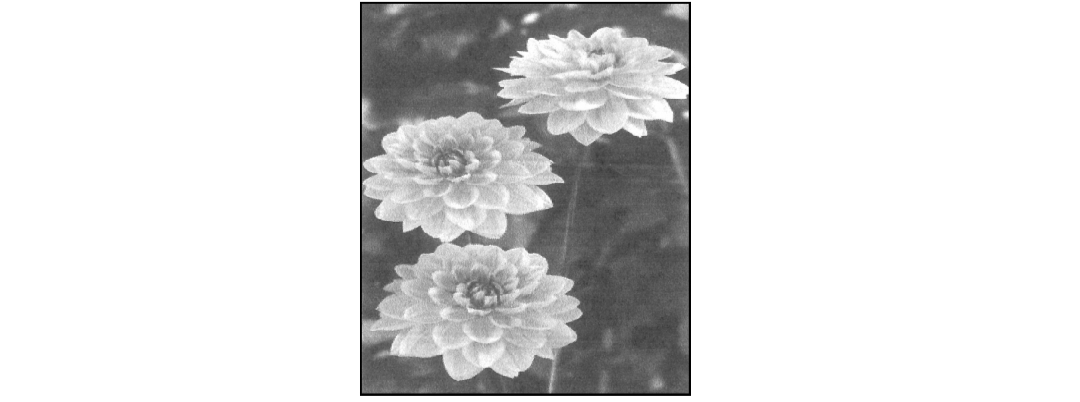
\includegraphics[width=\columnwidth]{figs/flowers}                                     
\caption{Three types of flowers}            
\label{fig:flowers11}                       
\end{figure}
\\ Based on  the above information :
\begin{enumerate}
\item  Calculate the probability that a randomly chosen seed will germinate.
\item  Calculate the probability  that the seed is of type $A_2$, given that a randomly choosen seed germinates.
\end{enumerate}
\item Three friends A, B and C got their photograph clicked. Find the probability that B is standing at the central position, given that A is standing at the left corner.
\item In a game of Archery, each ring of the Archery target is valued. The centremost ring is worth 10 points and rest of the rings are alloted points 9 to 1 in sequential order moving outwards.Archer A is likely to earn 10 points with a probability of 0.8 and Archer B is likely the earn 10 points with a probability of 0.9 \figref{fig:archery3} .
\begin{figure}[!ht]                     
\centering
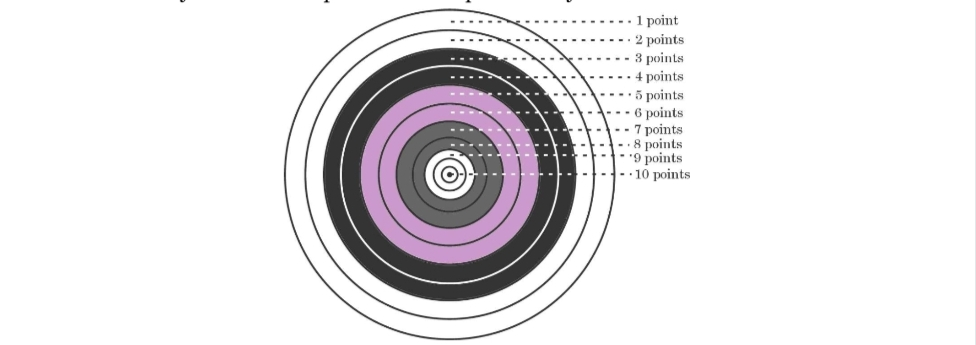
\includegraphics[width=\columnwidth]{figs/archery}
\caption{centermost ring}                   
\label{fig:archery3}                        
\end{figure}
\\ Based on the above innformation, answer the following questions :
\begin{enumerate}
\item exactly one of them earns 10 points .
\item both of them earn 10 point.
\end{enumerate}
\item Event A and B are such that \begin{align} P(A) = \frac{1}{2},  P(B) = \frac{7}{12}\end{align} and \begin{align} P(\bar{A}\cup \bar{B}) = \frac{1}{4} \end{align}
Find whether the events  A and B are independent or not.
\item A box $B_1$ contain 1 white ball  and 3 red balls. Another box $B_2$ contains 2 white balls and 3 red balls. If one ball is drawn at random from each of the boxes $B_1$ and $B_2$, then find the probability that the two balls drawn are of the same colour.
\item Let X be random variable which assumes values $x_1$, $x_2$, $x_3$, $x_4$  such that\begin{align} 2P(X = x_1) = 3P (X = x_2) = P ( X = x_3) = 5P (X = x_4).\end{align}
\\ Find the probability distribution of X.
\item There are two boxes, namely box-I and box-II. Box-I contains  3 red and 6 black balls. Box-II contains 5 red and 5 black balls. One of the two boxes , is selected at random and a ball is drawn at random. The ball drawn is found to be red. Find the probability that this red ball comes out from box-II.
\item In a toss of three different coins, find the probability of comming up of three heads, if it is known that at least one head comes up.
\item A laboratory blood text is $98\%$ effective  in detecting a certain disease when it is fact, present. However, the text also yeilds a false positive result for $0.4\%$ of the healthy person tested. From a large population, it is given that $0.2\%$ of the population actually has the diseases.
\\Based on the above, answer the following questtion : 
\begin{enumerate}
\item one person, from the population, is taken at random and given the test. Find the probabiliy of his getting a positive test result.
\item what is the probability that the person actually has the disease, given that his test result is positive ?
\end{enumerate}
\item Two cards are drawn from a well-shuffled pack of playing cards one-by-one with replacement. The probability that the first card is a king and the second card is a queen is 
\begin{enumerate}
\item $\frac{1}{13} + \frac{1}{13}$
\item $ \frac{1}{13} \times \frac{4}{51}$
\item $\frac{4}{52} \times \frac{3}{51}$
\item $\frac{1}{13} \times \frac{1}{13}$
\end{enumerate}
\item For two events A and B if P(A) = $\frac{4}{10}, P{B} = \frac{8}{10}$ and $P(B|A)$ = $\frac{6}{10}$ then find $P( A \cup B).$
\item Bag I contain 4 red and 3 black balls. Bag II contains 3 red and 5 black balls. One of two bags is selected at random and a ball is drawn from the bag, which if found to be red. Find the probability that the ball is drawn from bag II.
\item Two cards are drawn successively without replacement from a well-shuffled pack of 52 cards. Find the probability distribution of the number of aces and hence find its mean.
\item The probability of solving a specific question independently by A and B are $\frac{1}{3}$ and $\frac{1}{5}$ respectively . If both try to solve the question independently, the probability that the question is solved is 
\begin{enumerate}
\item $\frac{7}{15}$
\item $\frac{8}{15}$
\item $\frac{2}{15}$
\item $\frac{14}{15}$
\end{enumerate}
\item A card is picked at random from a pack of 52 playing cards. Given that the picked up card is a queen, the probability of it being a queen of spades is \underline{\hspace{1cm}}.
\item A bag contains 19 tickets, numbered 1 to 19. A ticket is drawn at random and then another ticket is drawn without replacing the first one in the bag. Find the probability distribution of the number of even numbers on the ticket.
\item Find the probability distribution of the numbers of successes in two tosses of a die, when a success is defined as number greater than 5.
\item Ten cartoons are taken at random from an automatic packing machine. The mean net weight of the ten carton is 11.8 kg and standard deviation is 0.15 kg. Does the sample mean differ significantly from the intended mean of 12 kg ?
[Given that for d.f. = 9, $t_{0.05}$ = 2.26]
\item A Coin is tossed twice. The following table \ref{tab: Number of tails} shows the probability distribution of numbers of tails:
\begin{table}[!ht]
\input{./2022/tablep.tex}	
\caption{Table shows the probability distribution of numbers of tails \label{tab: Number of tails}}
\end{table}
\begin{enumerate}
\item Find the value of $K$.
\item Is the coin tossed biased or unbaised?
Justify your answer.
\end{enumerate}
\item If X is a random variable with probability distribution as given below \ref{tab: probability distribution} :
\begin{table}[!ht]
\input{2022/tableb.tex}
\caption{table shows the proability distribution \label{tab: probability distribution}}
\end{table}
\newline The value of K and the mean of the distribution respectively are 
\begin{enumerate}
\item $\frac{1}{7}, 1$
\item $\frac{1}{6}, 2$
\item $\frac{1}{6}, 1$
\item $1, \frac{1}{6}$
\end{enumerate}
\item The random variable X has a probability function P($x$) as defined below, where K is some number :
\\ P(X)=$\begin{cases} K, & \text{if }  x=0 \\ 2K, & \text{if } x=1\\ 3K, & \text{if } x=2\\ 0, & \text{otherwise  } \end{cases}$ 
\\ Find:
\begin{enumerate}
\item The value of $K$.
\item $P(X<2),P(X \le 2), P(X \ge 2)$.
\end{enumerate}
\item Two rotten apples are mixed with 8 fresh apples. Find the probability distribution of number of rotten apples, if two apples are drawn at  random, one-by-one without replacement.
\end{enumerate}

\section{2023}
\subsection{10}
\input{2023/prob.tex}
\subsection{12}
\input{2023/probability12.tex}
\section{2022}
\subsection{12}
\begin{enumerate}
\item Let A and B be two events such that $P(A) = \frac{5}{8}$, $P(B) = \frac{1}{2}$ and  $P(A|B) = \frac{3}{4}$. Find the value of $P(B|A)$.
\item Two balls are drawn at random from a bag containing 2 red balls and 3 blue balls, without replacement. Let the variables X denotes the number of red balls. Find the probabillity distribution of X.
\item A card from a pack of 52 playing cards is lost. From the remaining cards, 2 cards are drawn at random without replacement, and are found to be both aces. Find the probability that lost card being an ace.
\item Probabilities of A and B solving a specific problem are $\frac{2}{3}$ and $\frac{3}{5},$ respectively. If both of them try independently to solve the problem, then find the probability that the problem is  solved.
\item A pair of dice is thrown. It is given that the sum of numbers  appearing on both dice is an even number. Find the probability that the number apprearing on at least one die is 3.
\item At the start of a cricket match, a coin is tossed and the team winning the toss has the opportunity to choose to bat or bowl. such a coin is unbaised with equal probabilities of getting head and tail \figref{fig:coin1} .
\begin{figure}[!ht]
\centering

\includegraphics[width=\columnwidth]{figs/coin}
\caption{Toss before the match}
\label{fig:coin1}
\end{figure}
\\ Based on the above information, answer the following question:
\begin{enumerate}
\item If such a coin is tossed 2 times, then find the probability distibution of numbers of tails.
\item Find the probability of getting at least one head in three tosses of such a coin.
\end{enumerate}
\item Two cards are drawn successively with replacement from a well shuffled pack of 52 cards. Find the probability distribution of the number of spade cards.
\item A pair of dice is thrown and the sum of the numbers appearing on the dice is observed to be 7. Find the probability that the number 5 has appeared on at least one die.
\item The probability that A hits the target is $\frac{1}{3}$ and the probability that B hits it, is $\frac{2}{5}.$ If both try to hit the target independently, find the probabillity that the target is hit. 
\item A shopkeeper sells three types of flower seeds A$_1$ , A$_1$ , A$_3$. They are sold in the form of a mixture, where the proportions of these seeds are  4 : 4 : 2, respectively. The germinaton rates of the three types of seeds are $45\%,$ $60\%$ and $35\%$ respectively \figref{fig:flowers11} .
\begin{figure}[!ht]
\centering                                  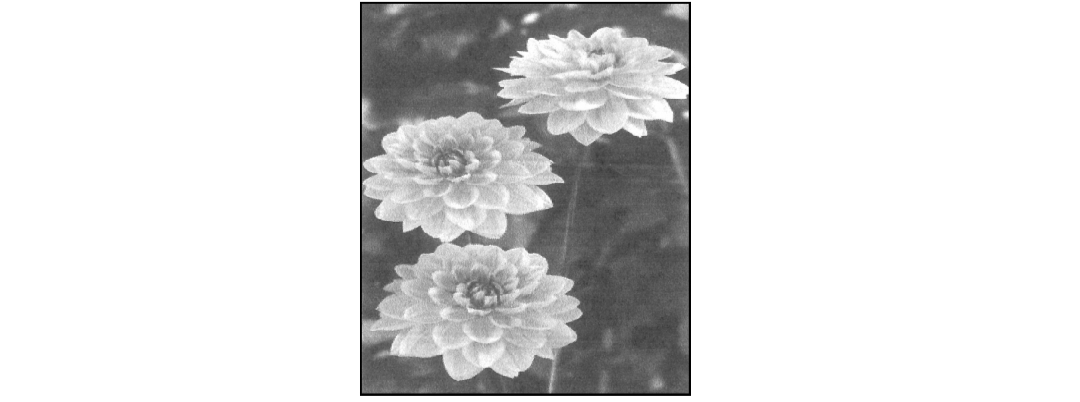
\includegraphics[width=\columnwidth]{figs/flowers}                                     
\caption{Three types of flowers}            
\label{fig:flowers11}                       
\end{figure}
\\ Based on  the above information :
\begin{enumerate}
\item  Calculate the probability that a randomly chosen seed will germinate.
\item  Calculate the probability  that the seed is of type $A_2$, given that a randomly choosen seed germinates.
\end{enumerate}
\item Three friends A, B and C got their photograph clicked. Find the probability that B is standing at the central position, given that A is standing at the left corner.
\item In a game of Archery, each ring of the Archery target is valued. The centremost ring is worth 10 points and rest of the rings are alloted points 9 to 1 in sequential order moving outwards.Archer A is likely to earn 10 points with a probability of 0.8 and Archer B is likely the earn 10 points with a probability of 0.9 \figref{fig:archery3} .
\begin{figure}[!ht]                     
\centering
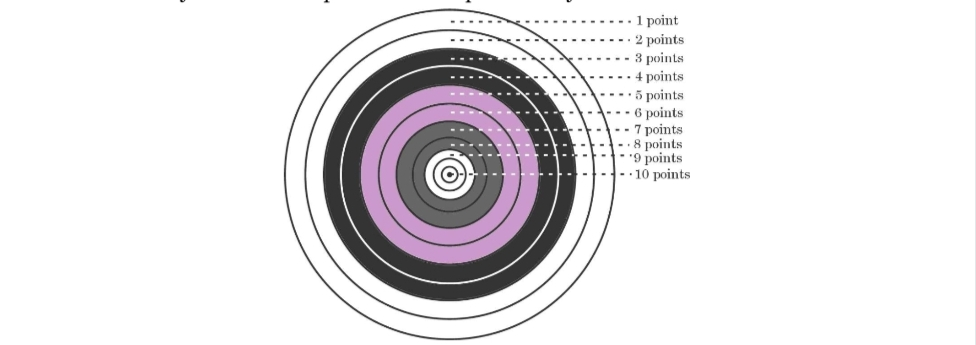
\includegraphics[width=\columnwidth]{figs/archery}
\caption{centermost ring}                   
\label{fig:archery3}                        
\end{figure}
\\ Based on the above innformation, answer the following questions :
\begin{enumerate}
\item exactly one of them earns 10 points .
\item both of them earn 10 point.
\end{enumerate}
\item Event A and B are such that \begin{align} P(A) = \frac{1}{2},  P(B) = \frac{7}{12}\end{align} and \begin{align} P(\bar{A}\cup \bar{B}) = \frac{1}{4} \end{align}
Find whether the events  A and B are independent or not.
\item A box $B_1$ contain 1 white ball  and 3 red balls. Another box $B_2$ contains 2 white balls and 3 red balls. If one ball is drawn at random from each of the boxes $B_1$ and $B_2$, then find the probability that the two balls drawn are of the same colour.
\item Let X be random variable which assumes values $x_1$, $x_2$, $x_3$, $x_4$  such that\begin{align} 2P(X = x_1) = 3P (X = x_2) = P ( X = x_3) = 5P (X = x_4).\end{align}
\\ Find the probability distribution of X.
\item There are two boxes, namely box-I and box-II. Box-I contains  3 red and 6 black balls. Box-II contains 5 red and 5 black balls. One of the two boxes , is selected at random and a ball is drawn at random. The ball drawn is found to be red. Find the probability that this red ball comes out from box-II.
\item In a toss of three different coins, find the probability of comming up of three heads, if it is known that at least one head comes up.
\item A laboratory blood text is $98\%$ effective  in detecting a certain disease when it is fact, present. However, the text also yeilds a false positive result for $0.4\%$ of the healthy person tested. From a large population, it is given that $0.2\%$ of the population actually has the diseases.
\\Based on the above, answer the following questtion : 
\begin{enumerate}
\item one person, from the population, is taken at random and given the test. Find the probabiliy of his getting a positive test result.
\item what is the probability that the person actually has the disease, given that his test result is positive ?
\end{enumerate}
\item Two cards are drawn from a well-shuffled pack of playing cards one-by-one with replacement. The probability that the first card is a king and the second card is a queen is 
\begin{enumerate}
\item $\frac{1}{13} + \frac{1}{13}$
\item $ \frac{1}{13} \times \frac{4}{51}$
\item $\frac{4}{52} \times \frac{3}{51}$
\item $\frac{1}{13} \times \frac{1}{13}$
\end{enumerate}
\item For two events A and B if P(A) = $\frac{4}{10}, P{B} = \frac{8}{10}$ and $P(B|A)$ = $\frac{6}{10}$ then find $P( A \cup B).$
\item Bag I contain 4 red and 3 black balls. Bag II contains 3 red and 5 black balls. One of two bags is selected at random and a ball is drawn from the bag, which if found to be red. Find the probability that the ball is drawn from bag II.
\item Two cards are drawn successively without replacement from a well-shuffled pack of 52 cards. Find the probability distribution of the number of aces and hence find its mean.
\item The probability of solving a specific question independently by A and B are $\frac{1}{3}$ and $\frac{1}{5}$ respectively . If both try to solve the question independently, the probability that the question is solved is 
\begin{enumerate}
\item $\frac{7}{15}$
\item $\frac{8}{15}$
\item $\frac{2}{15}$
\item $\frac{14}{15}$
\end{enumerate}
\item A card is picked at random from a pack of 52 playing cards. Given that the picked up card is a queen, the probability of it being a queen of spades is \underline{\hspace{1cm}}.
\item A bag contains 19 tickets, numbered 1 to 19. A ticket is drawn at random and then another ticket is drawn without replacing the first one in the bag. Find the probability distribution of the number of even numbers on the ticket.
\item Find the probability distribution of the numbers of successes in two tosses of a die, when a success is defined as number greater than 5.
\item Ten cartoons are taken at random from an automatic packing machine. The mean net weight of the ten carton is 11.8 kg and standard deviation is 0.15 kg. Does the sample mean differ significantly from the intended mean of 12 kg ?
[Given that for d.f. = 9, $t_{0.05}$ = 2.26]
\item A Coin is tossed twice. The following table \ref{tab: Number of tails} shows the probability distribution of numbers of tails:
\begin{table}[!ht]
\input{./2022/tablep.tex}	
\caption{Table shows the probability distribution of numbers of tails \label{tab: Number of tails}}
\end{table}
\begin{enumerate}
\item Find the value of $K$.
\item Is the coin tossed biased or unbaised?
Justify your answer.
\end{enumerate}
\item If X is a random variable with probability distribution as given below \ref{tab: probability distribution} :
\begin{table}[!ht]
\input{2022/tableb.tex}
\caption{table shows the proability distribution \label{tab: probability distribution}}
\end{table}
\newline The value of K and the mean of the distribution respectively are 
\begin{enumerate}
\item $\frac{1}{7}, 1$
\item $\frac{1}{6}, 2$
\item $\frac{1}{6}, 1$
\item $1, \frac{1}{6}$
\end{enumerate}
\item The random variable X has a probability function P($x$) as defined below, where K is some number :
\\ P(X)=$\begin{cases} K, & \text{if }  x=0 \\ 2K, & \text{if } x=1\\ 3K, & \text{if } x=2\\ 0, & \text{otherwise  } \end{cases}$ 
\\ Find:
\begin{enumerate}
\item The value of $K$.
\item $P(X<2),P(X \le 2), P(X \ge 2)$.
\end{enumerate}
\item Two rotten apples are mixed with 8 fresh apples. Find the probability distribution of number of rotten apples, if two apples are drawn at  random, one-by-one without replacement.
\end{enumerate}

\chapter{Construction}
\section{2023}
%\subsection{9}
\input{2023/construction-10th.tex}
\section{2022}
\subsection{10}
\begin{enumerate}
	\item In figure,\figref{fig:rightangled4} BN and CM are medians of a $\triangle$ ABC right-angled at A. Prove that \begin{align}4(BN^2 +CM^2) = 5BC^2\end{align} 
\begin{figure}[!ht]
\centering
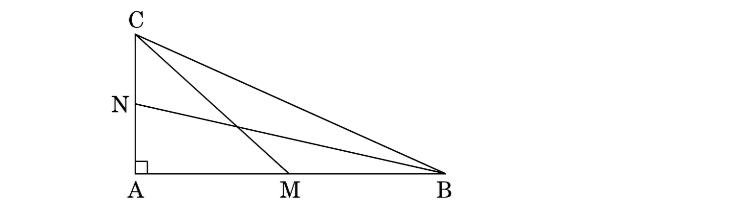
\includegraphics[width=\columnwidth]{figs/rightangled}
\caption{Right-angled triangle}
\label{fig:rightangled4}
\end{figure}
\item $\vec{Case Study - 1:}$
\begin{center}
$\vec{Kite Festival}$\\
\end{center}
Kite festival is celebrated in many countries at different times of the year. in India, every year 14th
January is celebrated as international kite Day. on his day many people visit India and participate in the festival by flying various kinds of kites.
\\The picture given below\figref{fig:kites5} , three kites flying together.
\begin{figure}[!ht]
\centering
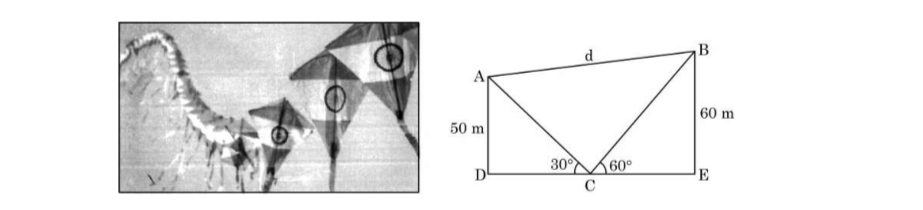
\includegraphics[width=\columnwidth]{figs/kites}
\caption{kites flying to gether}
\label{fig:kites5}
\end{figure}
\\In \figref{fig:kites5}, the angles of elevation of two kites (point C) are found to be $\degree{30}$ and  $\degree{60}$ respectively. Taking \begin{align}AD = 50 m\end{align} and\begin{align} BE = 60 m\end{align}
find 
\begin{enumerate}
\item The length of string used (take them straight) for kites A and B as shown in the figure.
\item The distance 'd' between these two kites
\end{enumerate}
\end{enumerate}
	

\section{2021}
\subsection{10}
\begin{enumerate}
	\item In figure,\figref{fig:rightangled4} BN and CM are medians of a $\triangle$ ABC right-angled at A. Prove that \begin{align}4(BN^2 +CM^2) = 5BC^2\end{align} 
\begin{figure}[!ht]
\centering
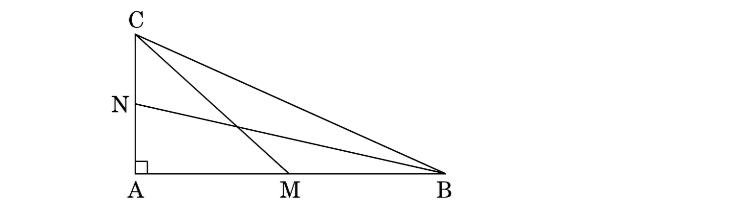
\includegraphics[width=\columnwidth]{figs/rightangled}
\caption{Right-angled triangle}
\label{fig:rightangled4}
\end{figure}
\item $\vec{Case Study - 1:}$
\begin{center}
$\vec{Kite Festival}$\\
\end{center}
Kite festival is celebrated in many countries at different times of the year. in India, every year 14th
January is celebrated as international kite Day. on his day many people visit India and participate in the festival by flying various kinds of kites.
\\The picture given below\figref{fig:kites5} , three kites flying together.
\begin{figure}[!ht]
\centering
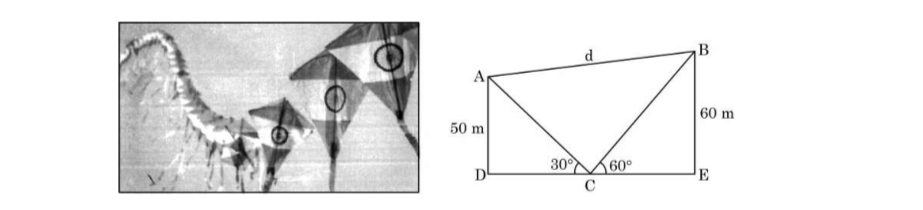
\includegraphics[width=\columnwidth]{figs/kites}
\caption{kites flying to gether}
\label{fig:kites5}
\end{figure}
\\In \figref{fig:kites5}, the angles of elevation of two kites (point C) are found to be $\degree{30}$ and  $\degree{60}$ respectively. Taking \begin{align}AD = 50 m\end{align} and\begin{align} BE = 60 m\end{align}
find 
\begin{enumerate}
\item The length of string used (take them straight) for kites A and B as shown in the figure.
\item The distance 'd' between these two kites
\end{enumerate}
\end{enumerate}
	

\chapter{Optimization}
\section{2023}
\input{2023/opti.tex}
%


%\include{ch02} 
\backmatter
\appendix
\iffalse
\chapter{Conic Lines}
\section{Pair of Straight Lines}
%
\input{quad/pair.tex}
\section{Intersection of Conics}
\input{quadlines/inter.tex}
\section{ Chords of a Conic}
\input{quadlines/chord.tex}
\section{ Tangent and Normal}
\input{quadlines/tangent.tex}
\fi
%\chapter{Proofs}
%   \section{}
%\input{apps/defs.tex}

%  \section{}
%\input{apps/parab.tex}
%  \section{}
%\input{apps/nonparab.tex}
%		\section{}
%\input{apps/params.tex}
\latexprintindex

\end{document}

 
\section{Examples}
\subsection{Loney}
\input{examples/loney.tex}
\subsection{Miscellaneous}
\input{examples/misc.tex}
%
%%\section*{Disclosure Statement}
%%The authors report there are no competing interests to declare.
%%
%%
%%
%%  
%%%All the results related to conics are summarized in 
%%%Table \ref{table:conics}.  
%%%\begin{table*}[!t]
%%%\centering
%%%\input{conics.tex}
%%%%\input{./figs/conics.tex}
%%%\caption{$\vec{x}^{\top}\vec{V}\vec{x}+2\vec{u}^{\top}\vec{x}+f = 0$  can be expressed in the above standard form for various conics. $\vec{c}$ represents the centre/vertex of the conic. $\vec{q}$ is/are the point(s) of contact for the tangent(s). }
%%%\label{table:conics}
%%%\end{table*}
%%%\begin{verbatim}
%%\bibliographystyle{tfs}
%%%\bibliography{interacttfssample}
%%\bibliography{school}
%%\end{verbatim}
%% included where the list of references is to appear, where \texttt{tfs.bst} is the name of the \textsc{Bib}\TeX\ bibliography style file for Taylor \& Francis' Reference Style S and \texttt{interacttfssample.bib} is the bibliographic database included with the \textsf{Interact}-TFS \LaTeX\ bundle (to be replaced with the name of your own .bib file). \LaTeX/\textsc{Bib}\TeX\ will extract from your .bib file only those references that are cited in your .tex file and list them in the References section.
%
%% Please include a copy of your .bib file and/or the final generated .bbl file among your source files if your .tex file does not contain a reference list in a \texttt{thebibliography} environment.
%

  % \section{Appendices}
  % \appendix
			\appendices
